\documentclass[reqno]{article}

\usepackage{fullpage}
\usepackage{eufrak}
\usepackage{listings}
\usepackage{color}
\usepackage{xcolor}
\usepackage{enumitem}


% \usepackage{nth}
\usepackage{amsthm,amsmath,amsfonts,amssymb}


%formatting
\usepackage[left=2cm,right=2cm,top=2cm,bottom=2cm,bindingoffset=0cm]{geometry}
\renewcommand{\baselinestretch}{1.2}
\sloppy


% Languages, fonts and symbols
\usepackage[english,russian]{babel}
\usepackage[T1,T2A]{fontenc}
\usepackage[utf8]{inputenc}
\usepackage{titlesec}

\usepackage{amsmath}

\usepackage{graphicx}
\graphicspath{{images/}} 
\DeclareGraphicsExtensions{.pdf,.png,.jpg}

\usepackage{subcaption}

\usepackage{amssymb}

\usepackage{listings}

\usepackage{float}

\usepackage{dsfont}

\usepackage{ragged2e}

\usepackage{tabularx}


%\usepackage{algorithm}
\usepackage[ruled,vlined]{algorithm2e}

\SetKwInput{KwInput}{Input}                % Set the Input
\SetKwInput{KwOutput}{Output}              % set the Output


% tikz graphics
% Для коммутативных диаграмм.
\usepackage{tikz}
\usetikzlibrary{arrows,shapes}
\tikzstyle{vertex}=[circle,fill=black,minimum size=3pt,inner sep=0pt]
\tikzstyle{edge} = [draw,thick,-]

\usepackage{tikz-cd}

\usetikzlibrary{quotes,babel,angles}


% Теоремы и прочее
\renewcommand\qedsymbol{$\square$}

\theoremstyle{definition}
\newtheorem*{nb}{Замечание}

\theoremstyle{definition}
\newtheorem*{sol}{Решение}

\theoremstyle{definition}
\newtheorem*{exmp}{Пример}

\theoremstyle{definition}
\newtheorem*{exmps}{Примеры}

\theoremstyle{definition}
\newtheorem{exc}{Упражнение}[section]

\theoremstyle{definition}
\newtheorem{thm}{Теорема}[section]

\theoremstyle{definition}
\newtheorem*{defi}{Определение}

\theoremstyle{definition}
\newtheorem{coll}{Следствие}[section]

\theoremstyle{definition}
\newtheorem{state}{Утверждение}[section]


%Content as links

\usepackage[hidelinks]{hyperref}
\hypersetup{
    colorlinks,
    citecolor=black,
    filecolor=black,
    linkcolor=black,
   urlcolor=black
}


% Title
\title{Математические модели микро- и макроэкономики.\\ Лекции.\\ ЧЕРНОВИК}
\author{Лектор: Мозговая К.А.\\ Автор конспекта: Курмазов Ф.А.\thanks{f.kurmazov.b@gmail.com}}
\date{\today}


% New Symbols
\newcommand*{\divby}{\mathrel{\rotatebox{90}{$\hskip-1pt.{}.{}.$}}}%

\begin{document}

	\setlength{\parindent}{0pt}
	\setlength{\parskip}{0.3em}
	
	\titleformat{\section}
	{\normalfont\Large\bfseries\newpage}
	{Лекция \thesection. }
	{0pt}{\Large}

	\maketitle

	\tableofcontents
	\newpage

	\section*{Макроэкономика}
		Макроэкономика - математическая модель, описывающая реальную картину мира, которая подтверждена или апробирована на тех данных, которые у нас есть.
		
		То есть основная идея макроэкономики заключается в \emph{жизненных проблемах}, связанных с некими экономическими показателями: зп, безработица, контракты между странами и др., но \emph{эти проблемы должны иметь четкую модель}, которая бы описывала любую такую взаимосвязь показателей. И при этом в настоящее время \emph{модель должна быть апробирована на данных} и должна прогнозировать. \medskip
		
		Проблемы могут тут возникнуть в том, как построить такую модель, как найти данные, как определить корректность данных... 
		
		Также стоит понимать, что макроэкономика неразрывно связанна с политикой. Например, модель \hyperref[sec:1.2]{экономического роста} $\rightarrow$ выпуск страны $\rightarrow$ конкурентная способность стран.
	
	\section{Роль человеческого капитала в моделях экономического роста. Модель Солоу}
		\subsection{Человеческий капитал}
			Человеческий капитал - экстерналия. Абсолютно невидимая вещь, которая приносит пользу обществу. То есть накопление нами знаний, умений, навыков, труда, невидимым образом повышает уровень развития общества.
			
			\begin{defi}
				Человеческий капитал — совокупность знаний, умений, навыков (существующие у каждого индивида), которые используются для удовлетворения многообразных потребностей общества в целом.
			\end{defi}
			
			Идея развития человеческого капитала идёт со времён Адама Смита, который говорил, что человеческий капитал - экстерналия, которую необходимо накапливать, чтобы разгонять технический прогресс в экономике.
			
			\begin{center}
				\emph{«Когда сооружается какая-нибудь дорогая машина, обыкновенно рассчитывают, что большое количество работы, которое она выполнит, пока не износится, возместит капитал, затраченный на нее по меньшей мере с обычной прибылью. Человек, изучивший с затратой большого труда и продолжительного времени какую-либо из тех профессий, которые требуют чрезвычайной ловкости и искусства, может быть сравнен с такою же дорогою машиною. Следует ожидать, что труд, которому он обучается, возместит ему, сверх обычной заработной платы за простой труд, все расходы, затраченные на, обучение, с обычной по меньшей мере прибылью на капитал, равный этой сумме расходов»}.
			\end{center}
			
			Человеческий капитал так же, как и физический, можно считать средством производства. Инвестиции в него приносят выгоду для общества в целом. И имеет место быть теория о том, что чем больше человеческого капитала, тем проще его накапливать. 
			
			В конце 20 века, в частности с развитием математических дисциплин (в том числе анализа данных, эконометрики...), экономисты пришли к выводу, что человеческий капитал, наряду с физическим, является неотъемлемым фактором современного экономического роста.
			
			С того момента в понятие человеческий капитал стали вносить также \textbf{здоровье, жизненный опыт и заботу о распорядке своего дня}. Ведь нанимать на работу здорового развитого человека лучше и выгоднее, чем нанимать того, на которого в будущем необходимо будет тратить деньги, чтобы лечить.
			
			Сейчас экономическая политика большинства развитых стран направлена увеличение инвестиций в человеческий капитал. Так как он сильно влияет на уровень выпуска в экономике и на темп его роста.  
			
			Ученые все время задаются вопросом, а как же измерить человеческий капитал? До сих пор никакой формализации нет, что придает этому фактору гибкости и универсальности, но также это приводит к дискуссиям и новым методам его измерения. 
		
		\subsection{Экономический рост}\label{sec:1.2}
		
		\begin{defi}
			Экономический рост - долгосрочная тенденция увеличения реального ВВП на душу населения в государстве.
		\end{defi}
		
		Чем выше темп экономического роста, тем выше уровень жизни в государстве. Калдор выделял \textbf{шесть факторов, которые должна включать в себя любая модель роста}:
		
		\begin{itemize}
			\item ВВП и производительность труда растут с течением времени;
			\item Величина физического капитала на одного рабочего растет во времени;
			\item Реальная ставка процента почти не меняется во времени (в развитых странах);
			\item Отношение запаса физического капитала к ВВП приблизительно постоянно;
			\item Доли заработных плат и дохода на капитал в структуре НД примерно постоянны;
			\item Темп роста выпуска на одного рабочего значительно отличается в разных странах.
		\end{itemize}
		
		В дальнейшем последовала колоссальная критика вышеперечисленных принципов. Тома Пикетти выпустил книгу "Капитал в XXI веке", в которой критиковалось отношение капитала к выпуску и критиковалась доля дохода на капитал. Он говорил, что доля должна демонстрировать всегда тенденцию к увеличению, а не к постоянству. Критика заключалась в том, что если доля всегда имела постоянный темп, то как выпуск на душу населения может расти, что тогда двигает этот рост становится не понятно.
		
		Несмотря на это, именно вышеперечисленные 6 постулатов Калдора заложили основу развития модели Солоу.
		
		\subsection{Модель Солоу}
		Модель Солоу -- модель экзогенного экономического роста. Она объясняет долгосрочный рост в экономике исключительно внешними факторами.
		
		\emph{Мы имеем выпуск, который задается неоклассической производственной функцией, зависящей от двух факторов производства} (труда и капитала). 
		
		$$Y_t=F(K_t,L_t)$$
		
		\textbf{Свойства $F(K,L)$}:
		\begin{enumerate}
			\item Постоянная отдача от масштаба 
			$$F(\lambda K, \lambda L) = \lambda F(K, L)$$
			
			\item Положительная и уменьшающаяся отдача от факторов производства
			$$\forall K,L > 0, F'_K (K, L) > 0, F'_L (K, L) > 0; F''_K (K, L) < 0, F''_L (K, L) < 0 $$
			$F'_K (K, L), F'_L (K, L)$ - предельная производительность труда и капитала соответственно.
			
			Т.е. мы не можем использовать $\infty$ - много какого-либо фактора производства, так как в какой-то момент увеличение этого фактора на единицу будет приносить снижение выпуска.
			
			Также мы не можем увеличивать один фактор, не изменяя другой (нам не нужно 100 ножек для стола, если крышек у нас всего 10).
			
			\item Условия Инады:
			\begin{itemize}
				\item Все факторы нужны для производства.
				$$\lim_{K \rightarrow 0} F'_K (K, L) = \lim_{L \rightarrow 0} F'_L (K, L) = \infty$$
				
				Мы не можем использовать только станки, оборудование...(капитал) и не использовать людей (труд). И наоборот.
				
				\item Выпуск растет при росте факторов производства.
				$$\lim_{K \rightarrow \infty} F'_K (K, L) = \lim_{L \rightarrow \infty} F'_L (K, L) = 0$$
				
				Чем больше мы используем труда и капитала, тем больше выпуск.
			\end{itemize}
		\end{enumerate}
		
		Также можно перейти к другой записи модели, пронормировав весь выпуск по количеству занятой рабочей силы.
		
		\emph{Капиталовооруженность труда}, т.е. величина капитала на одного рабочего $$k=\frac{K}{L}$$
		
		Соответственно у нас будет выпуск зависеть от капиталовооруженности: $f(k)$.
		
		Формулировка модели в величинах на душу населения удобна тем, что \emph{исключает зависимость от масштаба}: при постоянной капиталовооруженности $k$ увеличение или уменьшение населения (рабочей силы) не влияет на производительность.
		
		Описывая "репрезентативного" потребителя, нам будет не важно как он сформировался, но мы будем иметь его поведение, предпочтения, рабочую силу и доход, а также понимать, что он характеризуем общество в целом.
		
		В модели Солоу все потребители (агенты) друг от друга не отличаются, поэтому \emph{население можно считать единым "репрезентативным" потребителем}. Весь произведенный в периоде $t$ продукт после выплаты дохода на капитал и заработной платы оказывается сосредоточен у "репрезентативного" потребителя.
		
		Весь выпуск, который сосредотачивается у "репрезентативного" потребителя, приведен в некотором стоимостном выражении. Этот выпуск в денежном эквиваленте делится на потребление "репрезентативного" потребителя и его инвестиции.
		
		\begin{equation}\label{eq:1.3.1}
			Y_t = C_t + I_t
		\end{equation}
		
		Т.е. в каждый момент времени потребитель принимает решение, сколько он хочет потреблять (тратить деньги на товары, услуги, развлечения...), а сколько инвестировать (вложение в банк, ценные бумаги или под матрас... То есть то, что сейчас не тратится на потребление).
		
		В двухфакторной модели инвестиции можно назвать сбережениями.\bigskip
		
		На что направлены инвестиции? 
		
		Если посмотреть весь процесс, то наши сбережения попадают в банк, а впоследствии фирма берет кредит этого банка на развитие производства. Соответственно эти инвестиции формируют капитал:
		
		\begin{equation}\label{eq:1.3.2}
			K_{t+1} = (1 - \mu) K_t + I_t
		\end{equation}
		
		То есть капитал в каждый следующий период времени - это тот фактор производства, на который ориентируется фирма для того чтобы производить больше выпуска.
		
		Деньги от "репрезентативного" потребителя, которые не тратятся на потребление, направляются на развитие фирмы.  \emph{Соответственно уравнение \ref{eq:1.3.1} и \ref{eq:1.3.2} показывают, то, как много будет накапливаться капитала, для того чтобы увеличивался выпуск фирмы}. Если бы капитал не подлежал износу, то все деньги шли на развитие фирмы, но так как все наше оборудование изнашивается, это необходимо учесть (первое слагаемое уравнения \ref{eq:1.3.2}).
		
		Также у нас есть труд (вся рабочая сила, задействованная в производстве), который не является константой. Население растет, соответственно, вся рабочая сила изменяется из периода в период. 
		\begin{equation}\label{eq:1.3.3}
			L_{t+1} = (1 + n) L_t
		\end{equation}
		, где $n$ - темп роста населения
		
		Таким образом состояние экономики меняется из периода в период. Выпуск зависит от потребления в текущий период времени; от капитала, который мы хотим направить на развитие производства в будущий период времени и от того, сколько сейчас людей задействовано в производстве. 
		
		Соответственно наше решение сегодня (сколько потреблять, а сколько инвестировать) влияет на выпуск завтра. И темп роста населения сегодня влияет на то, сколько людей будет задействовано в развитии выпуска завтра. 
		
		Отсюда получаем, что вся модель является \emph{динамической}.\bigskip
		
		В моделях роста интересным является тот факт, как же выпуск $Y_t$ распределяется между потреблением $C_t$ и инвестициями $I_t$.
		
		Модель Солоу основана на самом простом предположении, что деление выпуска на потребление и валовые инвестиции осуществляется с помощью заданной извне и не меняющейся с течением времени нормы сбережения $s (0 < s < 1)$. 
		
		$$I_t = s Y_t$$
		$$K_{t+1} = (1 - \mu) K_t + s F(K_t, L_t)$$
		$$\frac{K_{t+1}}{L_{t+1}} = (1 - \mu) \frac{K_t}{L_{t+1}} + \frac{s F(K_t, L_t)}{L_{t+1}}$$
		
		\textbf{=> уравнение, задающее динамику в модели Солоу:}
		\begin{equation}\label{eq:1.3.4}
			(1 + n) k_{t + 1} = (1 - \mu) k_t + s f(k_t)
		\end{equation}
		
		Таким образом, если мы будем знать $k_0$, то мы будем знать весь выпуск из периода в период.
		
		Так как выпуск на душу населения задается:
		$$y_t = \frac{Y_t}{L_t} = f(k_t)$$
		Можно однозначно указать значения выпуска на душу населения $(y_t)_{t=0,1,\dots }$ и потребление на душу населения $(c_t)_{t=0,1,\dots}$ \bigskip
		
		\textbf{Траектория в модели Солоу} (исходящая из начального состояния $k_0$) - последовательность капиталовооруженностей и удельных потреблений $(k_t, c_t)_{t=0,1,\dots}$. Т.е. как менялась капиталовооруженность из периода в период.
		
		При отображении на графике мы будем видеть две независимые функции
		
		\begin{center}
			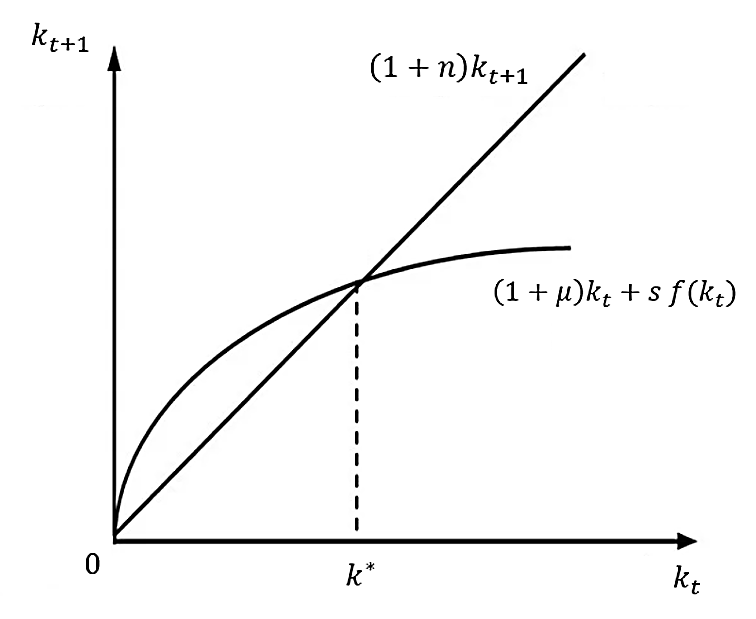
\includegraphics[width=0.35\textwidth]{Cтационарное_состояние_Солоу}
		\end{center}
		
		, где $k^*$ - это  точка стационарного состояния в системе. После неё не будет наблюдаться такого большого роста в экономике, который был до.
		
		Точка стационарного состояния в системе - некоторый уровень капиталовооруженности и потребления на душу населения, который не меняется с течением времени ($k^* = k_0^* = \dots = k_t^* = \dots; c^* = c_0^* = \dots = c_t^* = \dots$). 
		
		Тогда $$(n + \mu) k^* = s f(k^*)$$
		
		$k^*=0$ удовлетворяет равенству, при этом в силу условий Инады для производственной функции выполняется $f'(0) > n + \mu$
		
		Из сходимости последовательности капиталовооруженностей следует сходимость выпуска на душу населения к своему стационарному значению $f(k_t) \rightarrow f(k^*)$, а потребления к $c^* = (1-s)f(k^*)$. То есть удельные величины стабилизируются со временем, и это является той точкой, в которую пытается прийти любая динамическая система. 
		
		\textbf{Устойчивое состояние в системе} - максимально возможный капитал, максимально возможное потребление, которое мы можем добиться в нашей системе, если мы абстрагируемся от того, что существует индекс времени.
		
		Это теоретическая конструкция, без которой мы не можем говорить, что происходит на конкретных данных и как анализируются конкретные данные, посвященные накоплению капитала, потребления или данные, которые публикуются, связанные с ВВП.\bigskip
		
		От переменных капиталовооруженности мы можем перейти к переменным, которые описывают запас капитала в валовом исчислении. Получается мы переходим от удельных величин к валовым, и говорим какой объем капитала или выпуска мы ожидаем из периода в период. 
		
		$$\lim_{t \rightarrow \infty} \frac{K_{t+1}}{K_t} = \lim_{t \rightarrow \infty} \frac{Y_{t+1}}{Y_t} = 1 + n$$
		
		Никакое изменение параметров модели не может повлиять на постоянство удельных величин в долгосрочном периоде. Получается, что модель Солоу без технического прогресса не объясняет, откуда в долгосрочном периоде возникает рост на душу населения.
		
		Изменения $s,n,\mu$ или параметров производственной функции могут оказывать влияние только на уровни удельных переменных в стационарном состоянии.
		
		И именно предпосылка о константности нормы сбережения вызвала наибольшую критику модели Солоу. Эта предпосылка считается уникальной в своем роде, так как являлась неким прорывом в изучении моделях роста; но также она крайне неправдоподобна, так как не может из периода в период на инвестиции уходить фиксированная часть. Потому что все меняется, и меняется сама по себе суть модели, так как на принятие решения какую часть выпуска мы хотим отправить на инвестиции являются внешние факторы. Внешние факторы - шоки, которые из периода в период разные, поэтому и s не может быть стационарной. У нас должно быть написано уравнение, связывающее инвестиции и выпуск, и оно должно зависеть от многих факторов.
		
		\subsection{Модель Солоу с техническим прогрессом}
		
		Солоу сам говорил, что в его модели всегда будет рост и берется он с некоторого остатка. То есть Солоу предполагал, что существует набор факторов, который влияет на экономику.
		
		Последующие модели стали включать в себя, наряду с запасом физического капитала ($K_t$) и количеством труда ($L_t$), также параметр технического прогресса($A_t$)
		
		$$Y_t = A_t F(K_t,L_t)$$
		
		\textbf{Остаток Солоу (темп роста совокупной производительности факторов)} для функции Кобба-Дугласа:
		$$g^A = g^Y - \alpha g^K - (1 - \alpha) g^L$$
		, где
		
		$g^A$ - темп роста совокупной производительности факторов,
		
		$g^Y$ - темп роста выпуска,
		
		$g^K, g^L$ - темпы выпуска факторов производства,
		
		$\alpha, (1 - \alpha)$ - эластичности выпуска по факторам производства.
		
		\subsection{Последующие модели}
			Холодная война в 1960 годах заставила США разрабатывать стратегию роста, которая затмила бы СССР(основанную на двух параметрах $K$ и $L$).
			
			Так Шульц предложил повысить гос. расходы на образование. Которые, по его мнению, дадут США не только преимущество в гонке, но и обогатят человеческие ресурсы в целом, что повысит ее производительность.
			
			Фридман был не согласен и с Шульцом, и считал, что вложение в индивида будет пустой тратой денег. Так как возможно этот человек не хочет трудиться на благо страны, а  заботится только о себе.
			
			Он был только за индивидуальную свободу в обществе и капиталистическое предпринимательство. Индивид сам должен решать какое образование получать, или какой заработной платы он достоин на основании своих базовых знаний. То есть Фридман отрицал необходимости выдачи кредитов на образование, при этом индивиды должны были стать частными предпринимателями. И страна должна нанимать на работу не индивидов, а только частных предпринимателей. Ведь перевод рабочих в разряд независимых предпринимателей может укрепить в экономике регрессивную тенденцию рабочих договоров, в случае котором все издержки найма переходят на работника.  
			
			Таким образом Фридман и Шульц доказали важность человеческого капитала, доказали его влияние на экономический рост.
			
			Как же ученные строили модель роста учитывая человеческий капитал?
			
			\begin{itemize}
				\item \emph{Griliches Z.}
				
					Он предлагал включать $H$ как третий фактор производства. 
					$$Y = F(K,H,N)$$
					$H$-мера человеческого капитала, которая зависит от разности в заработных платах между квалифицированными работниками и "сырой" необразованной рабочей силой
					
					Кроме того, он говорил, что зарплата работников должна зависеть от квалификации самих работников.
					$$Y = F(K,EN)$$
					$L = EN$ (скорректированная относительно качества рабочая сила)
					$N$ - количество рабочих
					$E$ - индекс квалификации рабочей силы 
					
					В его теории нет фиксированных ставок зп. Чем  мы образованней, чем больше у нас $E$, тем больше у нас будет заработная плата.
					
					$$E = \sum_i r_i N_i/N$$
					$r_i$ - заработные платы работников для каждой $i$-ой категории
					
				\item \emph{Nelson R., Phelps E.}
				
					Nelson и Phelps же говорили, что человеческий капитал необходимо учитывать не отдельной третей переменной, а нужно добавить к L, некий индекс$A(t)$, характеризующий как на практике распространяются технологии.
					
					$$Y(t) = F \left(K(t),A(t)L(t)\right)$$
					$Y(t)$ -выпуск, производимый при таких параметрах;
					
					$K(t)$ - количество приобретенного в настоящее время капитала;
					
					$L(t)$ - количество нанятых работников, работающих с имеющимся капиталом;
					
					$A(t) = T(t-w(h))$ - технологический индекс (на практике). Он показывает интенсивность распространения технологии, т.е. он показывает временное запаздывание между развитием новой технологии и ее адаптацией на практике
					
					\setlength{\leftskip}{2em}
					$T(t)$ - теоретический уровень технологии;
					
					$w$ - уровень развития технологии, достигнутый год назад;
					
					$h$ -  уровень интенсивности/усовершенствования человеческого капитала
					
					\setlength{\leftskip}{0em}
					Т.е. готово ли конкретное производство подстроиться под инновации, обладает ли оно необходимым количеством людей для переобучения и внедрения новых технологических достижений.
					
					\begin{center}
						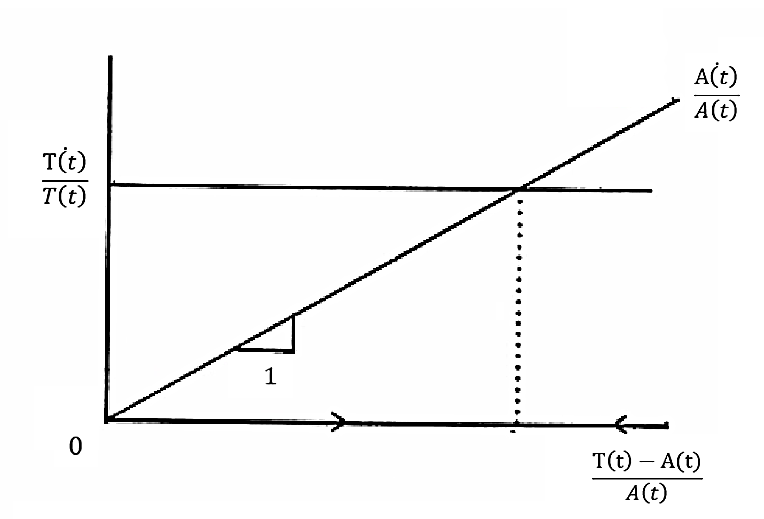
\includegraphics[width=0.4\textwidth]{Темп_распространения_технологий_на_практике}
						\label{Темп распространения технологий на практике}
					\end{center}
					
					$\dfrac{\dot{T(t)}}{T(t)}$ - темп развития теоретического уровня технологии
					
					$\dfrac{\dot{A(t)}}{A(t)}$ - темп распространения технологии на практике
						
					$\dfrac{T(t)-A(t)}{A(t)}$ - разрыв между теоретическим уровнем технологии и уровнем технологии на практике
					
				\item \emph{Romer P.}
				
					Он говорит, что существует взаимосвязь между человеческим капиталом и изменением темпов роста в сравнении между странами. А также, что наблюдается эффект влияния образования на уровень инвестиций. Темп роста инвестиций, в свою очередь, имеет положительную устойчивую связь с темпом роста экономики.
					
					Тогда возникает вопрос, а как же выявить эффект влияния образования на уровень инвестиций и как его использовать.
					
					По его мнению, существенную роль в техническом развитии и развитии выпуска, играют инновации и государственные затраты на НИОКР. Если затрат не будет, то и не будет технического роста.
					
					Индивид должен обладать тремя разных навыками для того, чтобы он был полезен государству (для наращивания выпуска):
					
					\begin{itemize}
						\item Физические $(L_i)$: координация, сила
						
						\setlength{\leftskip}{2em}
						Инвестиции в питание, здоровье...
						
						\setlength{\leftskip}{0em}
						\item Образовательные $(E_i)$: полученные в начальной и средней школе
						
						\setlength{\leftskip}{2em}
						Измеряются количеством полных лет обучения
						
						\setlength{\leftskip}{0em}
						\item Способность к научной/исследовательской деятельности $(S_i)$ ("научный талант")
						
						\setlength{\leftskip}{2em}
						Навыки, отличающие выпускников колледжа от ученых, инженеров от рабочих технических специальностей
						
					\end{itemize}
					
					$Y(L^Y, E^Y, X^Y) = \dot{K} + C$ - общий объем выпуска
					
					$ \dot{K} $ - темп прироста капитала;
					
					$ C $ - общий объем потребления;
					
					$ X^Y $ - описывает технологический процесс, который начинается на этапе изготовления "макетов" и заканчивается на стадии выпуска готовой продукции.
					
					Если предприятие не будет нанимать людей, которые обладают этими тремя навыками, то оно не сможет внедрять те инновационные разработки, которые есть уже на рынке и соответственно будет терять свою конкурентоспособность.
					
					Чем определяется эксклюзивность продукта?
					
					\begin{itemize}
						\item Конкурентоспособный товар
						
						Потребитель руководствуется собственными предпочтениями
						
						\item Неконкурентоспособный товар
						
						Дополнительные технические или законодательные ограничения вынуждают потребителя приобретать данный товар
					\end{itemize}
					
					Ромер доказывает если вы можете изобретать конкурентоспособный товар, то у вас наращивается производство. И чем больше разного конкурентоспособного товара в стране, тем больше будет наблюдаться уровень ВВП. Получается, что главная действующая сила - люди, обладающие научным талантом.
					
					Государству необходимо развивать этот научный талант за счет обучения, поднятия уровня знаний, уровня распространения знаний, уровня начальных разработок. Таким образом, важно чтобы в стране создалась среда, которая позволяла бы каждому индивиду использовать все имеющиеся знания и их направлять на практику.
					
					Таким образом Ромер доказал и апробировал на данных то, что важно развивать человеческий капитал.
					
				\item \emph{Lucas R.}	
				
					Его основная идея заключается в том, что темпы обучения в школе, на работе зависят не только от собственных усилий человека, но и в решающей степени от людей, с которыми взаимодействует.
					
					Соответственно, наше семья, наше окружение влияет на то, готовы ли мы и хотим ли вообще накапливать человеческий капитал или нет.
					
			\end{itemize}
			
			\textbf{ВЫВОДЫ:}
			
			\begin{itemize}
				\item \emph{Smith A.}: Навыки и умения, полученные работниками (например, в ходе обучения, тренировки) могут повысить экономическую ценность предприятия;
				
				\item \emph{Nelson R.}: Образованные люди совершают инновации, таким образом, образование ускоряет процесс развития технологий;
				
				\item \emph{Griliches Z.}:Дальнейшее образовательное движение работника не может быть ограничено только "пулом" его прошлых способностей;
				
				\item \emph{Lucas R.}: Чем выше уровень людей, с которыми Вы работаете, тем больше Вы выучите и больших навыков приобретете.
			\end{itemize}
			
			
	\section*{Дз 1.}
		\begin{exc}
			Имеется два типа товаров. Пусть известны цены на товары $p_x, p_y$, при этом $x, y$ - количество товаров 1-го и 2-го типов соответственно, $x,y \geq 0$. Доход потребителя ограничен и равен $m > 0$. Предположим, предпочтения потребителя описаны фукнцией полезности $u(x,y) = x + \alpha y, \alpha > 0.$
			
			Найти решение оптимизационной задачи. Какое условие нужно сформулировать, чтобы задача имела решение при $x,y > 0$.
		\end{exc}
		
		Метод лагранжа.
		
		Теорема Куна-Теккера.
		
		Функция полезности.
		
		Выпуклые/Вогнутые функции.
		
		Chapter 2,3 из книги Varian.
		
		Knut Sydsæter, Peter Hammond Essential Mathematics for Economic Analysis (fourth edition), Глава 8, Chapter 13, 14.
		
		План на следующую субботу: 
		
		Лекция 1 - обсудим оптимизационные задачи и метод Лагранжа
		
		Лекция 2 - задача потребительского выбора и функция полезности
		
	\section{}

\end{document}


% Examples and Shortcuts

	\begin{defi}
	Определение чего-то
	\end{defi}


	\begin{thm}

	\end{thm}	


	\begin{coll}

	\end{coll}	

	
	\begin{nb}

	\end{nb}	

	
	\begin{nb}

	\end{nb}	


	\begin{exmp}

	\end{exmp}	


	\begin{tikzcd}
	A \arrow[rd] \arrow[r, "\phi"] 
	&B \\
	& C \arrow[u]
	\end{tikzcd}

	% Пример мат. постановки

	$$\text{min} \quad \sum\limits_{e \in E} x_e$$
	
	$$
	\text{s.t.}
	\begin{cases}
		\sum\limits_{e \in E_v} x_e \geq 1& \forall v \in V\\
		x \in \{0, 1\}^{|E|} &
	\end{cases}
	$$

	% Пример алгоритма

	\begin{algorithm}[H]
		\SetAlgoLined
		 \SetKwFunction{FDFS}{DFS}
		 \SetKwProg{Fn}{Function}{:}{}
		 \Fn{\FDFS{$u$}}{
			$VisitFunc(u)$\;
			$visited[u] = True$\;
		        \For{$w \in \text{adj}[u]$}
						{
							\If{$visited[w] = False$}
								{
								$FoundFunc(w)$\;
								$\text{DFS}(w)$\;
								}						
							}
			$OutFunc(u)$\;
		        }

		DFS(start)
		\caption{Depth-first search}
	\end{algorithm}
